\documentclass[UTF8]{ctexart}
\usepackage{graphicx}
\usepackage{listings}

\title{实验二报告}
\author{唐灵\\519030910052\\F1903002}
\date{\today}
\begin{document}
    \maketitle
    \begin{abstract}
        这是电工导c课程的第二次实验
    \end{abstract}
    \section{实验概览}
        本次实验主要针对网络爬虫,关键技术包括利用cookie进行登陆,爬虫的深度优先,广度有限策略,
        利用哈希函数和哈希表进行字符串是否存在于集合内的快速判断,多线程技术等等。
        最终的目的是利用以上的所有技术实现大规模的数据爬取。(当然有礼貌也是很重要的)
    \section{实验环境}
    本次实验的所有代码在电类工程导论c课程中在课程方统一给定的“ee208”$Docker$容器中运行并实现。
    \section{练习解决思路}
        \subsection{练习一的解决思路}
            练习一要求实现BloomFilter,我们选择把Bitarray类作为子类,实现BloomFilter类。在初始化函数中就可以直接通过传入
            的参数n(希望存储的字符串大致个数),按照理论直接产生相对合适的哈希函数个数,和二值表大小。\par
            类中具有self.k(哈希函数个数),self.m(二值表大小),self.bitarray(二值表对象)三个属性。\par
            hash\_str()(基于BKDRHash)方法用于产生并使用不同的哈希函数来对于每一个字符串进行哈希运算得到哈希值。
            使用两个函数分别进行检查单词是否存在于表格内,和往哈希表中添加元素。\par
            这样我们就实现了满足了基本的一些要求。

            值得一提的是,对于BKDRHash函数,对于哈希表的大小很有讲究,如果设定为非素数的话,最终的错误率会提高很多个量级,
            我的做法是将输入的n,一般为10底的指数,加上1,作为最终的大小,这样就满足了设定为素数,得到较为理想的结果。
        \subsection{练习二的解决思路}
            实现爬虫过程,事实上只需要将返回页面内容的函数,以及从页面内容中提取url的函数完善即可。\par
            针对第一个函数,如果是需要爬取有登陆页面的网页,就必须利用cookie(partA中所练习的)进行登陆,
            这里图简单就选择了一些简单的网页进行爬取,所以直接返回即可。值得一提的是由于爬取的是中文网页,
            所以应该采用utf-8的解码方式进行解码。否则将会返回一些乱码(如果url中不含中文的话实际上对于问题的解决也影响不大)\par

            针对第二个函数,由于我们的任务比较简单,所以直接采用正则表达式对于字符串进行匹配,不再采用bs(为了提升效率),这样当然也会带来一些问题,
            比如匹配的不精确,正则并不是万能的。\par

            这两个函数都采用了try,和except,保证了容错率。
        \subsection{练习三的解决思路}
            练习三强调了多线程,代码框架基本给出,一些基本函数都可以用上一个练习的成果。\par
            这时遇到最大的困难在于对于多线程运行框架的理解——具体问题体现在,如何让这个爬虫在爬取到一定的数量的页面之后就停止爬取,
            我们都知道用个人电脑无限爬取是荒谬的。\par
            首先应该对于q.join()函数的实质进行理解,用大白话来说,当判断q.join()为0时主线程结束,若子线程都是守护线程,随着主线程结束,
            都会被强制结束掉,所以问题的关键在于将跳出条件和join关联起来,put()操作可以让join()+1(摔了一个锅),
            get()和task\_down()形成一对时才能让join()-1,通俗来说,接了一个锅要完成了才能行,没完成,任务量是不会减的。\par
            有了这个通俗的认识,我们的想法是,对于已经爬取的元素进行计数,当爬去元素的个数刚好超过预期时,
            就把q清空(也必须用很多对get(),task\_done()来完成),这时候就自然跳出了.\par
            除了这个点,有些变量在运行过程中需要上锁也是值得注意的。
    \section{代码运行结果}
        \subsection{练习一的运行结果}
            对于练习一,我们的测试方式是,随机生成1000个长度为12的字符,放进Fillter之中,
            之后独立实验20次,每一次独立实验,都再次随机生成10000个长度为12的字符,
            检查是否存在于Fillter之中,如果存在,记为一次失误(因为12的长度保证了概率上产生于之前字符相同的字符的
            概率极其的小),最终计算失误率,再对20次实验取平均值,得到最终的实际误差率,进行打印并进行比较。结果如下:
            \begin{figure}[ht]
                \centering
                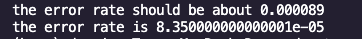
\includegraphics[scale=0.75]{img/error.png}
                \caption{练习一程序运行结果}
            \end{figure}
            
            可以看出结果是比较理想的。
        \subsection{练习二的运行结果}
            练习二的运行结果存储在html文件夹,以及index.txt文件之中,打印出来信息如下:
            \begin{figure}[ht]
                \centering
                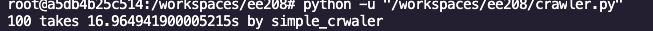
\includegraphics[scale=0.5]{img/sim.png}
                \caption{练习二程序运行结果}
            \end{figure}
        \subsection{练习三的运行结果}
            练习三的运行结果存储在html文件夹,以及index.txt文件之中,打印出来信息如下:
            \begin{figure}[ht]
                \centering
                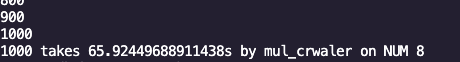
\includegraphics[scale=0.5]{img/mul.png}
                \caption{练习三程序运行结果}
            \end{figure}

            对比于上一个练习,可以容易看出,对于线程为8的情况,多线程爬虫能够提高接近于两倍的效率。
            多线程针不戳!
    \section{分析与思考}
    \begin{enumerate}
        \item 练习二中给出的代码是dfs,函数就是dfs,做的也是dfs,由于队列是类似dfs所以可能是想方便作对比吧,个人觉得在小范围爬的时候其实广度有限应该能够获取更多的信息,会更好一点。
        \item 将fillter融入爬虫只需要将已经爬去列表改成我们创造的类,然后修改相应的增加和检查函数,是容易的,这里在crwaler\_final.py进行了实现,
        由于提高了搜索效率,这种方法在大数据量,以及更多的线程上相对于普通的多线程会更加具有优势。
        \item 这个问题没有进行探索,电工导任务量确实有点大。
        \item 这显然是不可能的,因为线程与线程之间要共用一些变量,一个在用的时候,另一些变量是不能用的,打个比方,大家想进学校搬东西,是不是人越多越好呢,在人都能轻松进入校门的时候,人当然越多越好,但是当人大到一定程度,
        我希望进入学校,但是根本挤不进去,这时候能够被搬出来的东西就有限了,即使我非常想为学校服务都做不到,线程的增多对于效率的提升是有限的。
        \item 以后可以探索
    \end{enumerate}
    \begin{figure}[ht]
        \centering
        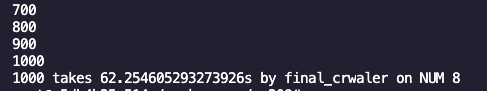
\includegraphics[scale=0.5]{img/num8.png}
        \caption{8线程运行时间}
    \end{figure}
    \begin{figure}[ht]
        \centering
        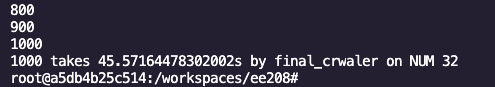
\includegraphics[scale=0.5]{img/num32.png}
        \caption{32线程运行时间}
    \end{figure}
    \begin{figure}[ht]
        \centering
        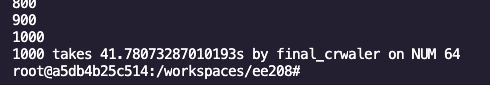
\includegraphics[scale=0.5]{img/num64.png}
        \caption{64线程运行时间}
    \end{figure}
    \begin{figure}[ht]
        \centering
        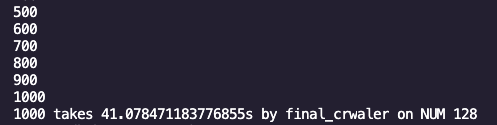
\includegraphics[scale=0.5]{img/num128.png}
        \caption{128线程运行时间}
    \end{figure}

    
    ———线程的增加对于效率的提升是有限的。
\end{document}